\subsection{Virtual Machines}
\begin{frame}
    \frametitle{Virtualization vs. Physical}
    \begin{itemize}
        \item Benefits of virtual machine (VM) technology
            \pedbullet{Fast and economical solution for lab environment deployment}
            \pedbullet{Network segregation can be virtualized}
            \pedbullet{Pre-infection system restore is painless}
        \item Pitfalls of virtual machine (VM) technology
            \pedbullet{Malware can detect the VM and alter behaviour}
            \pedbullet{Virtualization \emph{may} have bugs in replication of physical system}
        \item Should have at least one physical system in a malware lab
    \end{itemize}
    \begin{columns}
    \column{.7\textwidth}
        \begin{itemize}
            \item CoreRESTORE (www.coreprotect.com)
            \item Provides hardware level reboot-to-restore functionality
        \end{itemize}
    \column{.3\textwidth}
        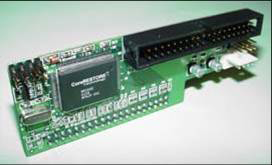
\includegraphics[scale=.40]{images/vms_and_live_analysis/corerestore.png} \\
    \end{columns}
\end{frame}

\begin{frame}
    \frametitle{x86 Virtual Machine Capabilities}
    \begin{itemize}
        \item x86 architecture does not meet Popek and Goldberg virtualization requirements
        \item Virtualization is accomplished via dynamic recompilation (like Java)
        \item This isn't all that important to know, just know that dynamic recompilation is slower than true self-virtualization
        \item AMD "Pacifica" and Intel "Vanderpool" have architecture level support for virtualization
    \end{itemize}
    \pedref{ACM-17-7}
\end{frame}

\begin{frame}
    \frametitle{Virtualization vs. Emulation}
    \begin{itemize}
        \item VM technologies such as VMware trap all hardware access and simulate the entire motherboard minus the processor
        \item Emulation technologies such as Bochs completely emulate the processor, hardware devices and memory
        \item Emulation is slower but provides greater flexibility of control and "safety" in terms of malware "breaking out" of the controlled environment
        \item Partial emulation can be very helpful in static analysis
    \end{itemize}
\end{frame}

\begin{frame}
    \frametitle{Virtual Machine Technologies}
    \begin{itemize}
        \item \alert{VMware}
            \pedbullet{VMWare server is now free}
        \item Microsoft Virtual PC (Connectix)
            \pedbullet{This is also free}
        \item Microsoft Virtual Server
        \item Plex86
        \item Xen
        \item Parallels
    \end{itemize}
\end{frame}

\begin{frame}
    \frametitle{Emulation Technologies}
    \begin{itemize}
        \item Bochs
            \pedbullet{The Bochs instrumentation library is badass, as Ero will show later}
        \item Qemu
        \item Chris Eagle's IDA x86-emu plug-in (partial emulation)
    \end{itemize}
\end{frame}


\begin{frame}
    \frametitle{VMWare Tips}
    \tip{Use a USB/Firewire disk for increased performance}
    \tip{Save snapshot disk space by installing new software from the network or CD}
\end{frame}


\subsection{Live Analysis}
\begin{frame}
    \frametitle{What and Why?}
    \begin{definition}
        Simply put, live analysis constitutes of running suspect code in a "sacrificial" environment while monitoring its activities at a high level
    \end{definition}

    \begin{itemize}
        \item Live analysis falls well short of reverse engineering
        \item However, it is still the most frequently used analysis technique
        \item A good starting point for "unfolding" the story
    \end{itemize}
\end{frame}

\begin{frame}
    \frametitle{SysInternals}
    \begin{itemize}
        \item SysInternals is home of Marc Russinovich
        \item Offers a number of excellent freeware and commercial utilities
        \item You know Marc from the Sony rootkit debacle
        \item More recently you may have heard of them due to the Best Buy Geek Squad scandal
        \item Most recently you may have heard of them because they sold to Microsoft
    \end{itemize}
\end{frame}

\begin{frame}
    \frametitle{SysInternals RegMon}
    \begin{itemize}
        \item Monitor all registry access in real time
        \item Supports filtering
    \end{itemize}
    \begin{center}
        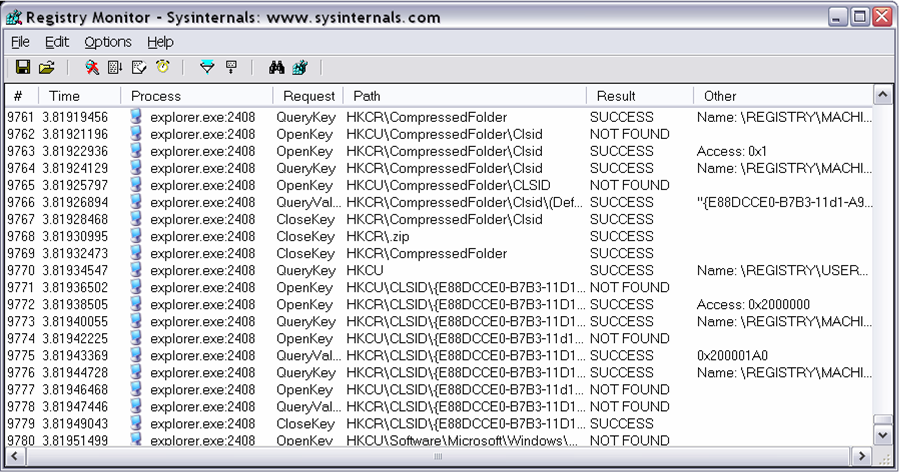
\includegraphics[scale=.35]{images/vms_and_live_analysis/regmon.png}
    \end{center}
\end{frame}

\begin{frame}
    \frametitle{SysInternals FileMon}
    \begin{itemize}
        \item Monitor all file access in real time
        \item Supports filtering
    \end{itemize}
    \begin{center}
        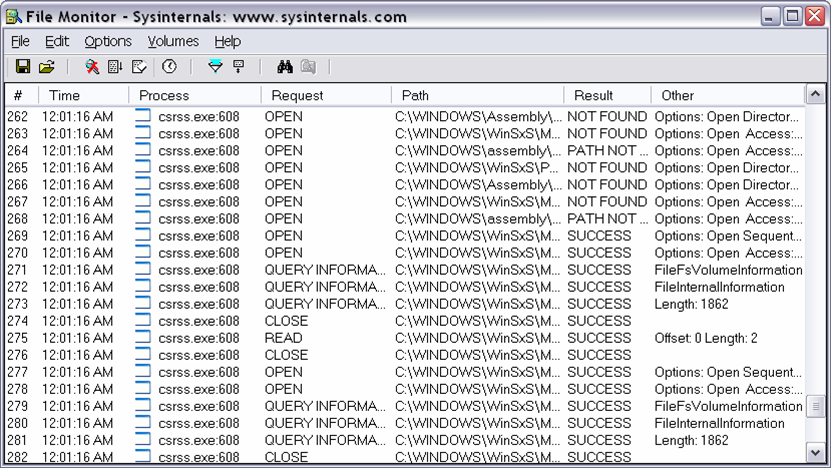
\includegraphics[scale=.35]{images/vms_and_live_analysis/filemon.png}
    \end{center}
\end{frame}

\begin{frame}
    \frametitle{SysInternals TCPView}
    \begin{itemize}
        \item Monitor all per-process socket endpoints in real time
            \pedbullet{ie: Determine what ports a specific process is bound to}
        \item Supports filtering
    \end{itemize}
    \begin{center}
        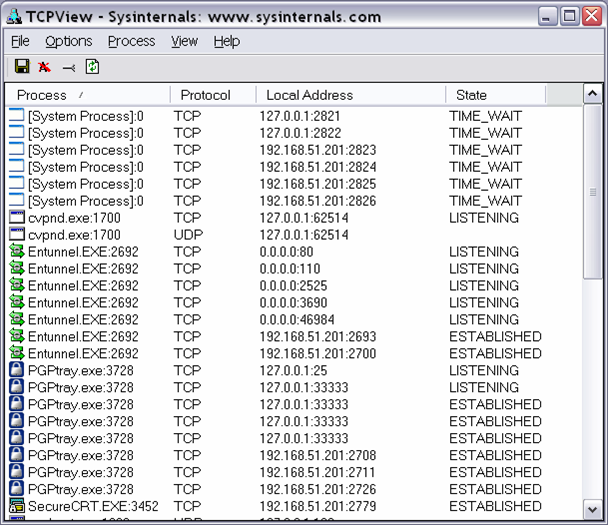
\includegraphics[scale=.30]{images/vms_and_live_analysis/tcpview.png}
    \end{center}
\end{frame}

\begin{frame}
    \frametitle{SysInternals Process Explorer}
    \begin{itemize}
        \item Task manager on steroids
        \item Exposes a plethora of useful information
    \end{itemize}
    \begin{center}
        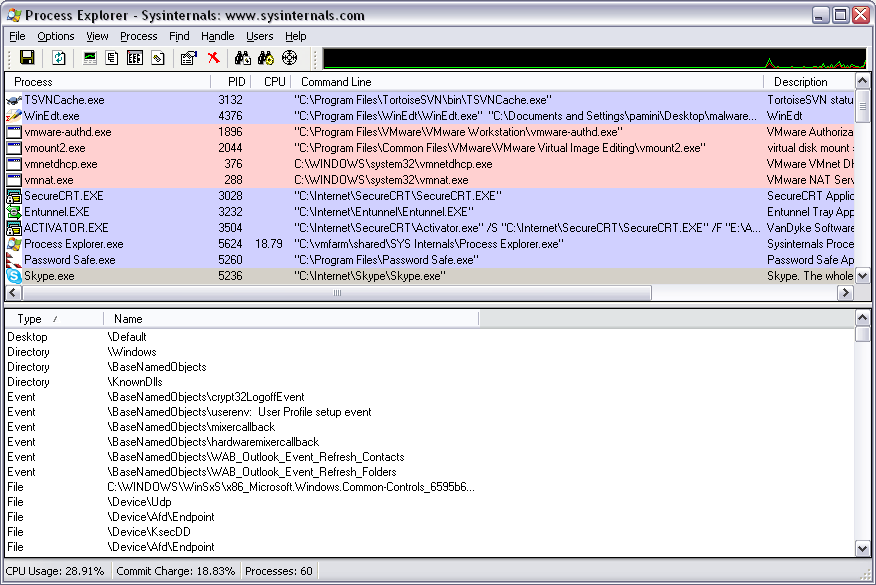
\includegraphics[scale=.30]{images/vms_and_live_analysis/process_explorer.png}
    \end{center}
\end{frame}

\begin{frame}
    \frametitle{InCtrl}
    \begin{columns}
    \column{.5\textwidth}
        \begin{itemize}
            \item Originally designed to monitor changes made by installers
            \item Applies well to malware
            \item Takes system "snapshots" pre/post execution
            \item Generates HTML report of monitors changes
        \end{itemize}
    \column{.5\textwidth}
        \begin{center}
            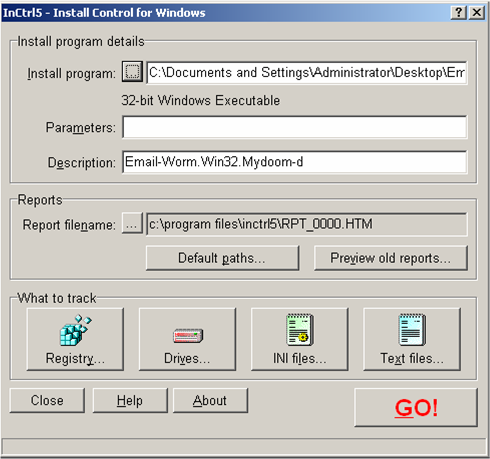
\includegraphics[scale=.5]{images/vms_and_live_analysis/inctrl.png} \\
        \end{center}
    \end{columns}
\end{frame}

\begin{frame}
    \frametitle{Wire Shark / Ethereal}
    \begin{columns}
    \column{.5\textwidth}
        \begin{itemize}
            \item Formerly known as Ethereal
            \item Wonderful and free network sniffer
            \item Can decipher a number of protocols
            \item Also vulnerable, very vulnerable
        \end{itemize}
    \column{.5\textwidth}
        \begin{center}
            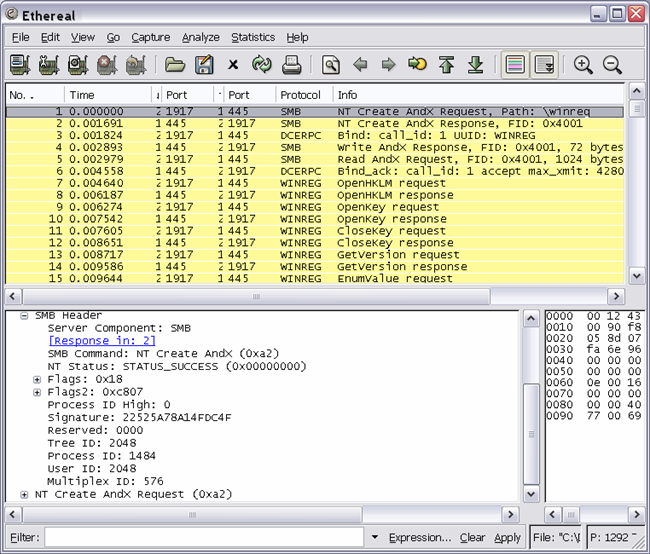
\includegraphics[scale=.30]{images/vms_and_live_analysis/ethereal.png} \\
        \end{center}
    \end{columns}
\end{frame}

\begin{frame}
    \frametitle{Dave Zimmer's Tools}
    \begin{itemize}
        \item Who is Dave Zimmer?
            \pedbullet{A VB coding machine}
            \pedbullet{His tools are currently available from http://labs.idefense.com}
        \item Malcode Analyst Pack
            \pedbullet{FakeDNS, IDCDumpFix, Mailpot, SCLog, ShellExt, Sniffhit, SocketTool}
        \item Multipot
            \pedbullet{Emulation based honeypot}
        \item SysAnalyzer
            \pedbullet{Like InCtrl, but specifically designed for malware}
    \end{itemize}
\end{frame}